% chapter 9
% Last edit: 2017-5-4
\chapter{Inferences Based on Two Samples}
\section{$z$ Tests and Confidence Intervals for a Difference Between Two Population Means}

\[X_1,\dots,X_n \overset{iid}{\sim} N(\mu_1,\sigma_1^2), \sigma_1 \text{ known}.\]
\[Y_1,\dots,Y_n \overset{iid}{\sim} N(\mu_2,\sigma_2^2), \sigma_2 \text{ known}.\]

\begin{prop}
\[E(\bar{X}-\bar{Y})=\mu_1-\mu_2\]
\[Var(\bar{X}-\bar{Y})=\frac{\sigma_1^2}{n}+\frac{\sigma_2^2}{n}\]
\end{prop}

\subsection{Test Procedures for Normal Populations with Known Variances}
Case I
\[Z=\frac{\bar{X}-\bar{Y}-(\mu_1-\mu_2)}{\sqrt{\frac{\sigma_1^2}{n}+\frac{\sigma_2^2}{n}}} \sim N(0,1)\]

$H_0:\mu_1-\mu_2=\Delta_0$
\begin{enumerate}
\item With $H_a: \mu_1-\mu_2>\Delta_0$, $RR:Z\geq z_{\alpha}$.
\item With $H_a: \mu_1-\mu_2<\Delta_0$, $RR:Z\leq -z_{\alpha}$.
\item With $H_a: \mu_1-\mu_2\neq\Delta_0$, $RR:|Z|\geq z_{\alpha/2}$.
\end{enumerate}

\begin{exmp}
(Example 9.1 in textbook)
\end{exmp}

\subsection{Large-Sample Tests}
Case II large sample, $\sigma^2$ unknown

\[Z=\frac{\bar{X}-\bar{Y}-(\mu_1-\mu_2)}{\sqrt{\frac{S_1^2}{n}+\frac{S_2^2}{n}}} \sim N(0,1)\]

$100(1-\alpha)$ CI for $\mu_1-\mu_2$
\[ \bar{X}-\bar{Y} \pm z_{\alpha/2} \sqrt{\frac{S_1^2}{n}+\frac{S_2^2}{n}} \]

\section{The Two-Sample $t$ Test and Confidence Interval}
Case III

(a) 

\[X_1,\dots,X_n \overset{iid}{\sim} N(\mu_1,\sigma_1^2)\]
\[Y_1,\dots,Y_n \overset{iid}{\sim} N(\mu_2,\sigma_2^2)\] 

$\sigma_1,\sigma_2 \text{ independent} $

\[T=\frac{\bar{X}-\bar{Y}-(\mu_1-\mu_2)}{\sqrt{\frac{S_1^2}{n}+\frac{S_2^2}{n}}} \sim t(\nu) \qquad \nu=\frac{\left( \frac{S_1^2}{n}+\frac{S_2^2}{n} \right)^2}{ \frac{\left( \frac{S_1^2}{m} \right)^2}{m-1}+ \frac{\left( \frac{S_1^2}{m} \right)^2}{n-1}  } \]

$100(1-\alpha)$ CI for $\mu_1-\mu_2$
\[\bar{X}-\bar{Y} \pm t_{\alpha/2,\nu} \sqrt{\frac{S_1^2}{n}+\frac{S_2^2}{n}}  \]

\[H_0:\mu_1-\mu_2=\Delta_0 \qquad T=\frac{\bar{X}-\bar{Y}-\Delta_0}{\sqrt{\frac{S_1^2}{n}+\frac{S_2^2}{n}}} \sim t(\nu)\]
\begin{enumerate}
\item With $H_a: \mu_1-\mu_2>\Delta_0$, $RR:T\geq t_{\alpha,\nu}$.
\item With $H_a: \mu_1-\mu_2<\Delta_0$, $RR:T\leq -t_{\alpha,\nu}$.
\item With $H_a: \mu_1-\mu_2\neq\Delta_0$, $RR:|T|\geq t_{\alpha/2,\nu}$.
\end{enumerate}

\begin{exmp}
(Example 9.6 in textbook)
\end{exmp}

\subsection{Pooled $t$ Procedures}
(b) Small sample size, $\sigma_1^2=\sigma_2^2$

\[T=\frac{\bar{X}-\bar{Y}-(\mu_1-\mu_2)}{\sqrt{\frac{S_p^2}{n}+\frac{S_p^2}{n}}}\]

\[S_p=\frac{n-1}{m+n-2}S_1^2+\frac{m-1}{m+n-2}S_2^2\]

"pooled sample variance"

\[S_1^2=\frac{1}{n-1} \sum_{i=1}^n (X_i-\bar{X})^2 \qquad S_2^2=\frac{1}{m-1} \sum_{i=1}^m (Y_i-\bar{Y})^2 \]

\begin{exmp}
Body weight gained on animal treatment: given 1 mg/piller dose of soft steroid control: placebo.
% what is the word 
\begin{center}
\begin{tabular}{l|c|c|c}
\hline
treatment & $m=8$ & $\bar{x}=32.8$ & $s_1=2.6$ \\
\hline
placebo & $n=8$ & $\bar{y}=40.5$ & $s_2=2.5$ \\
\hline
\end{tabular}
\end{center}

Does the data suggest the average weight gain in the control group exceeds that in the treatment group by more than 5 g? $\alpha = 0.01$

\begin{enumerate}
\item $H_0:\mu_1-\mu_2 = -5 \qquad H_a:\mu_1-\mu_2 < -5$
\[T^*=\frac{\bar{X}-\bar{Y}-(-5)}{\sqrt{\frac{S_1^2}{n}+\frac{S_2^2}{n}}}=-2.23 \]
\[\nu=\frac{\left( \frac{S_1^2}{n}+\frac{S_2^2}{n} \right)^2}{ \frac{\left( \frac{S_1^2}{m} \right)^2}{m-1}+ \frac{\left( \frac{S_1^2}{m} \right)^2}{n-1}  }=\frac{\left(\frac{2.6^2}{8}+\frac{2.5^2}{10}\right)^2}{\frac{1}{7} \left(\frac{2.6^2}{8}\right)^2+\frac{1}{9} \left(\frac{2.5^2}{10}\right)^2}=14.886 \approx 14\]
\[P-Value=P(T_{14}\leq T^*)=0.022>0.1\]
\item Assume $\sigma_1^2=\sigma_2^2$

$H_0:\mu_1-\mu_2 = -5 \qquad H_a:\mu_1-\mu_2 < -5$

\[T^*=\frac{\bar{X}-\bar{Y}-(-5)}{\sqrt{\frac{S_p^2}{n}+\frac{S_p^2}{n}}}=-2.24\]
Here $S_p=\sqrt{\frac{2.6^2 (8-1)}{8+10-2}+\frac{2.5^2 (10-1)}{8+10-2}}=2.54$

\[P-Value=P(T_{16}<-2.24)=0.021>0.01\]

\end{enumerate}
\end{exmp}

\section{Analysis of Paired Data}
$n$ independent selected pairs
$(X_1,Y_1),(X_2,Y_2),\dots,(X_n,Y_n)$

\[E(X_i)=\mu_1 \qquad E(Y_i)=\mu_2\]
\[H_0:\mu_1-\mu_2=\Delta \qquad H_a:\mu_1-\mu_2 \neq\Delta\]
\begin{center}
\begin{tabular}{ccccc}
\hline
$X$ & $X_1$ & $X_2$ & \dots & $X_n$ \\ 
$Y$ & $Y_1$ & $Y_2$ & \dots & $Y_n$ \\ 
$D=X-Y$ & $D_1=X_1-Y_1$ & $D_2=X_2-Y_2$ & \dots & $D_n=X_n-Y_n$ \\
\hline
\end{tabular}
\end{center}

\[H_0:\mu_D=\mu_1-\mu_2=\Delta \qquad H_a:\mu_D=\mu_1-\mu_2 \neq\Delta\]
\[D_1,D_2,\dots,D_n\]

\[T=\frac{\bar{D}-\Delta}{S_D/\sqrt{n}}\]
\[\bar{D}=\frac{1}{n}\sum_{i=1}^n D_i \qquad  S_D^2=\frac{1}{n-1}\sum_{i=1}^n (D_i-\bar{D})^2\]

\subsection{The Paired $t$ Test}

\begin{exmp}
(Exercise 8.39 in textbook) reports the accompanying data on amount of milk ingested by each of 14 randomly selected infants.

Does it appear that the true average difference between intake values measured by the two methods is something other than zero? Determine the $P$-value of the test, and use it to reach a conclusion at significance level 0.05.

\end{exmp}

$100(1-\alpha)$\% CI for $\mu_1-\mu_2=\mu_0$
\[\bar{D} \pm t_{\alpha/2,n-2}\frac{S_D}{\sqrt{n}}\]

\section{Inferences Concerning a Difference Between Population Proportions}

\begin{prop}
Let $X\sim Bin(n,p_1)$, $Y\sim Bin(m,p_2)$ with $X$ and $Y$ independently. $\hat{p_1}=\frac{X}{n}$,$\hat{p_2}=\frac{Y}{m}$
\[E(\hat{p_1}-\hat{p_2})=p_1-p_2\]
\[Var(\hat{p_1}-\hat{p_2})=\frac{p_1(1-p_1)}{n}+\frac{p_2(1-p_2)}{m}\]
\end{prop}

As $n$ and $m$ get larger,
\[Z=\frac{\hat{p_1}-\hat{p_2}-(p_1-p_2)}{\sqrt{\frac{p_1(1-p_1)}{n}+\frac{p_2(1-p_2)}{m}}} \overset{iid}{\sim} N(0,1)\]

$100(1-\alpha)$\% CI for $p_1-p_2$
\[\hat{p_1}-\hat{p_2} \pm z_{\alpha/2}\sqrt{\frac{\hat{p_1}(1-\hat{p_1})}{n}+\frac{\hat{p_2}(1-\hat{p_2})}{m}}\]

\subsection{A Large-Sample Test Procedure}

To test $H_0$: $p_1-p_2=0$

Test statistic: \[Z=\frac{\hat{p_1}-\hat{p_2}-0}{\sqrt{\hat{p}(1-\hat{p}) \left(\frac{1}{n}+\frac{1}{m} \right)}}\] 

where $\hat{p}=\frac{X+Y}{n+m}$

\begin{enumerate}
\item With $H_a: p_1-p_2>0$, $RR:Z \geq z_{\alpha}$.
\item With $H_a: p_1-p_2<0$, $RR:Z \leq -z_{\alpha}$.
\item With $H_a: p_1-p_2\neq 0$, $RR:|Z|\geq z_{\alpha/2}$.
\end{enumerate}


\begin{exmp}
\begin{tabular}{c|c|c}
\hline
	& plea guilty & plea not guilty \\ \hline
Judged guilty	& $m=191$ & $n=64$ \\ \hline
Sentenced to prison & $x=101$ & $y=56$ \\ \hline
\end{tabular}

\[H_0: p_1-p_2=0 \qquad p_1\neq p_2\]
\[\hat{p_1}=\frac{101}{191}=0.53 \qquad \hat{p_2}=\frac{56}{64}=0.875\]
\[Z=\frac{\hat{p_1}-\hat{p_2}-0}{\sqrt{\hat{p}(1-\hat{p}) \left(\frac{1}{n}+\frac{1}{m} \right)}} \qquad \hat{p}=\frac{101+56}{191+64}=0.616\] 
\[Z^*=-4.91 \qquad RR:\{|Z|\geq z_{\alpha/2}=2.58\} \quad \alpha=0.01\]
\[Z^* \in RR \Rightarrow \text{Reject }H_0\]

Conclusion:
% conclusion is needed
\end{exmp}

\section{Challenge Question 4}
\begin{figure}[H]
\centering
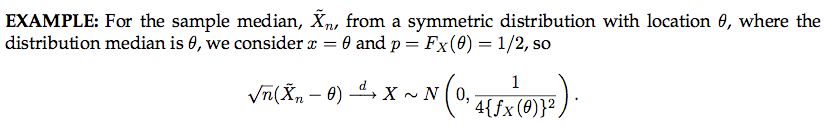
\includegraphics[scale=0.5]{median.jpeg}
\end{figure}

\begin{proof}
\[\lim_{n \to\infty} P(\sqrt{n}(\tilde{X_n}-\theta)\leq a)=P(Z \leq 2 f(\theta)a)\]

Let $Y_i=I\left(X_i\leq \theta+\frac{a}{\sqrt{n}}\right) \qquad i=1,2,\dots,n$
\[Y_i=\begin{cases}
1, & x_i\leq \theta+\frac{a}{\sqrt{n}} \\
0. & x_i\geq \theta+\frac{a}{\sqrt{n}} 
\end{cases}\]

Clearly, $Y_1,Y_2,\dots,Y_n \overset{iid}{\sim} Bern(p_n)$

\[p_n=P\left(X_i\leq \theta+\frac{a}{\sqrt{n}}\right)=F\left( \theta+\frac{a}{\sqrt{n}}\right)\]

\begin{align*}
P(\sqrt{n}(\tilde{X_n}-\theta)\leq a)= & P\left(\tilde{X_n}\leq \theta+\frac{a}{\sqrt{n}}\right)\\
= & P\left( \sum_{i=1}^{n} Y_i \geq \frac{n+1}{2} \right) \\
= & P\left(\frac{\sum_{i=1}^{n} Y_i -n p_n}{\sqrt{n p_n(1-p_n)}} \geq \frac{\frac{n+1}{2} -n p_n}{\sqrt{n p_n(1-p_n)}}\right)
\end{align*}

Note that $p_n \to\frac{1}{2}, n\to \infty$. By CLT,

\[ \frac{\sum_{i=1}^{n} Y_i -n p_n}{\sqrt{n p_n(1-p_n)}}  \overset{d}{\to} N(0,1)\]

\[\lim_{n\to\infty} \frac{F\left(\theta+\frac{a}{\sqrt{n}}-F(\theta)\right)}{a/\sqrt{n}}=F'(\theta)=f(\theta)\]

\[\frac{n\left(p_n-\frac{1}{2}\right)}{\sqrt{n}} \longrightarrow f(\theta)\cdot a\]

\[\frac{np_n-\frac{n+1}{2}}{\sqrt{n}} \longrightarrow f(\theta)\cdot a \qquad \sqrt{p_n(1-p_n)} \longrightarrow \frac{1}{2} \qquad n\to\infty\]

\[\frac{\frac{n+1}{2} -n p_n}{\sqrt{n p_n(1-p_n)}}\longrightarrow -2af(\theta)\]
\end{proof}

Another proof: Bootstrap.
\begin{proof}
$X_1,\dots,X_n \overset{iid}{\sim} f(x)$. Distribution of $\tilde{X_n}$. Bootstrap: if $f(x)$ is "known".

\begin{align*}
\tilde{X_n^{(1)}} \leftarrow & X_1^{(1)} \dots X_n^{(1)} \overset{iid}{\sim} f(x)  \\
\tilde{X_n^{(2)}} \leftarrow & X_1^{(2)} \dots X_n^{(2)} \overset{iid}{\sim} f(x)  \\
\tilde{X_n^{(3)}} \leftarrow & X_1^{(3)} \dots X_n^{(3)} \overset{iid}{\sim} f(x)  \\
\dots\dots & \dots\dots\dots\dots\dots\dots \\
\tilde{X_n^{(B)}} \leftarrow & X_1^{(B)} \dots X_n^{(B)} \overset{iid}{\sim} f(x)  
\end{align*}
\[\tilde{f(x)}=\frac{1}{n} \qquad \text{if } x=x_i\]

Sample $n$ values from $\{x_1,\dots,x_n\}$ with replacement.
\end{proof}